\section{Schematic}\label{sec:schematic}

The main board was drawn in KiCad 10.0.4 entirely through the Konnect MCP server. No agent edited a KiCad file as text. The current release, \textbf{v0.2}, includes the readability redraw, a root block diagram with sheet pins, ECO-001 and ECO-002 \src{hw/mainboard/BUILD_NOTES.md}. It has 271 parts on nine sheets (\cref{tab:sheets}); 12 of them are DNP. \Cref{fig:sch-root,fig:sch-rails,fig:sch-mcu,fig:sch-amp} reproduce four pages. The full PDF is \repo{hw/mainboard/out/speaker_main_schematic.pdf}.

\begin{checked}
\begin{itemize}[leftmargin=1.2em,itemsep=1pt]
  \item \textbf{Against the spec:} RefDes coverage was checked by script, and every IC, transistor and connector was checked pin by pin using the nets read back from KiCad.
  \item \textbf{ERC:} 0 violations at all severities, no exclusions. One caveat: the CH340C symbol hides +3V3's real driver, so that net was confirmed in the netlist.
  \item \textbf{After every edit} (redraw, root rework, ECO-001, ECO-002), the netlist was compared with the previous release. Only the intended changes appeared.
  \item \textbf{Reviews:} an independent review and two skill-driven release reviews, v0.1 and the v0.2 delta. They covered pins against pads, footprints against drawings, boundary states and supply. Verdict: \textbf{no blockers}; the open items are in \cref{app:register}.
\end{itemize}
\end{checked}

\textbf{Still to do before fabrication:}
\begin{itemize}
  \item Set KiCad's DNP attribute on the 12 parts; Konnect cannot set it.
  \item Confirm the XT30 polarity on a real part.
  \item Plan placement of the three tall electrolytics.
  \item Fix the small documentation leftovers in \cref{sec:inconsistencies}.
\end{itemize}

\newcommand{\schpage}[3]{%
\begin{figure}[p]
\centering
\includegraphics[page=#1,angle=90,width=0.97\linewidth,height=0.86\textheight,keepaspectratio]{speaker_main_schematic.pdf}
\caption{#2}\label{#3}
\end{figure}}

\schpage{1}{Schematic v0.2, root sheet: the KiCad version of \cref{fig:power-path,fig:data-path}. The power path runs along the top (USB, charger, battery, rails, amplifiers); the data path runs below (USB-UART, MCU, UI link, amplifiers). The blue bus carries I\textsuperscript{2}C, AMP\_PDN, the fault lines, I\textsuperscript{2}S and CHG\_QON.}{fig:sch-root}

\schpage{5}{Page 5, \texttt{rails}. Top: the TPS61178 boost with the ECO-001 compensation (\qty{100}{\kilo\ohm}/\qty{15}{\nano\farad}) and the trim network R907/D901, now fitted for the soft start. Bottom: the TPS62933 buck to +3V3. The text blocks are the design notes the build agent placed on each sheet.}{fig:sch-rails}

\schpage{6}{Page 6, \texttt{mcu}. The ESP32-WROVER-E with every usable GPIO assigned, the I\textsuperscript{2}C pull-ups, the \qty{2.2}{\micro\farad} EN capacitor, the \qty{68}{\ohm} SPI/PDM source resistors, the two-FET fault merge and test points TP105--TP110.}{fig:sch-mcu}

\schpage{9}{Page 9, \texttt{amp\_left}. The TAS5805M in BTL with its address strap (0x2C), PVDD decoupling, bootstrap capacitors and the four \qty{10}{\micro\henry} + \qty{1}{\micro\farad} output legs to the woofer (channel A) and tweeter (channel B). The right amplifier (page 10) differs only in RefDes, strap and test points.}{fig:sch-amp}

\clearpage
